\chapter{Training process of Convolutional Neural Networks}\label{ch:cnn_train}
Three Convolutional Neural Networks (CNNs) were trained throughout this analysis. There are differences to each CNN and will be described fully in the next sections but the main difference are the amount of particle images used for training and validation. CNN1075 used 1,075 muons and 1,075 pions for training and the same amout of each particle for validation. CNN10000 used 10,000 muons and 10,000 pions split in half for testing and training. Lastly CNN100000 had muons, pions, protons, electrons, and gammas in it's training and validation set. Each particle had 20,000 images and training and validation was split $90\%$ training, $10\%$ validation. This chapter will also describe the different hardware frameworks used for training beginning on a CPU and ending on a GPU cluster. 


%\section{Hardware Frameworks used for Training}
%\subsection{Syracuse CPU Machine setup}
%\subsection{Syracuse University GPU Cluster Setup}


\section{Hardware Configurations for Convolutional Neural Network Training}\label{research approach}
The first training iteration, CNN1075, was a proof of concept. This CNN was trained on my local machine for \sim 4-5 weeks. The batch size had to be very small as well as the image size due to the lack of compuation resources. The second iteration of training, CNN10000, was trained on a Fermilab stationed Syracuse University machine. This machine had 6 TB of disk space, 6 cores at 2.1 GHz and 32 GB of RAM. The use of this machine allowed me to increase the training sample as well as the batch size and hence further increase the accuracy of the neural network. Lastly, the CNN100000 was trained using two GTX 1080 Ti GPUs with 11GB of memory on a node on the Syracuse University GPU cluster, SUrge, that has 8 cores and 16GB of memory. This increase in memory as well as the capability to use 2 GPUs drastically cut down on training time from \sim 4-5 weeks to \sim 8 hours. SUrge also allowed for hyperparameter optimization by being able to run mulitple training iterations over the two GPUs. Lastly, SUrge allowed for training over higher resolution images and a larger particle class of 5 particles vs 2 particles. 

\section{Creating images using LArTPC data for training/validation of CNNS}\label{image_making}
The $\mu/\pi$ image dataset used to train and validate CNN1075 was created using single generated isotropic muons and pions from 0-2 GeV energy range. 2,150 muons and 2,150 pions were used for training and testing split 50\%. The images were created using LArSoft, a liquid argon software, and were based on wire number and time tick in the collection plane. Uboonecode reconstruction version v05{\_}08{\_}00 was used. The raw ADC value after noise filtering was the wire signal. Each collection plane greyscale image was 3456x1600x1 where 6 time ticks were pooled into 1 bin. 

After the image was created, the region of interest (ROI) in the image was found by using Open CV, a image processing open source software package, to scan the image starting from the edges and stopping once a bright pixel is encountered. At this step, the ROI can be larger or smaller than the necessary size of a training image and the XY ratio of the image is not kept. This ROI is then resized to an image of 224x224x1. 

The greyscale color standard is 8bit therefore the ADC value of wire and time tick was also downsampled due to the 12bit ADC value MicroBooNE has. To do this, the highest ADC pixel in the image was found and then this was divided by the rest placing all pixel values between 0-1. From there, all pixel values are then multiplied by 255.

The $\mu/\pi$ image dataset used to train and validate the CNN10000 was also created using single generated isotropic muons and pions from 0-2 GeV energy range. 10,000 muons and 10,000 pions were used for training and testing split 50\%. Uboonecode v06{\_}23{\_}00 was used instead of v05{\_}08{\_}00. Each collection plane greyscale image was 3456x1280x1 where 5 time ticks were pooled into 1 bin which is different than the previous dataset and was implemented due to the fact that the time ticks of an event went from 9400 to 6400 with the change of uboonecode version. Issues that arose in CNN1075 that were fixed in CNN10000 include zero-padding images in X and Y that are smaller than 224X224 to eliminate over-zooming effect and fixing a bug that shifted pixels separated by a dead-wire region.

The $\mu/\pi/p/e/\gamma$ image dataset used to train and validate the CNN100000 were created using single generated isotropic particles with energy range from 0-2 GeV. 20,000 of each particle were used for training and were split 90/10 between training and testing sets. Uboonecode v06{\_}23{\_}00 was used for these images. The collection plane greyscale iamge had the same dimensions as CNN10000, 3456x1280x1 and the ROI algorithm was the same except for resizing these images to 576x576. 

A major change other than the higher resolution images was the treatment of the ADC values. In the first two image making schemes, the highest pixel value was found per image and the image was then normalized by that. The issue arising from this ADC normalization wasn't inherent in $\mu/\pi$ training due to the fact that both particles are minimum ionizing particles in liquid argon, however, when dealing with a larger particle class, it was necessary to try and make sure energy deposition by each particle was preserved. The energy deposition in a particle image corresponds to the ADC value or pixel brightness. To preserve energy deposition, the ADC float value was passed straight to the image rather than doing any image normalization. This then makes sure that minimum ionizing particles like muons and pions appear dimmer than highly ionizing particles like protons.  

Images were also made from BNB+Cosmic events that passed the cc-inclusive selection 1 filter right before the 75 cm track length cut and were classified using the CNN10000. The dataset used to create these images is the same one used in \cite{cc-inclusive}, \textit{prodgenie{\_}bnb{\_}nu{\_}cosmic{\_}uboone{\_}mcc7{\_}reco2}. These images were created using information from the track candidate that passed the filter. Only wire number and time ticks associated to the track candidate were drawn on the image to mimic a single particle generated image. 

These images were then classified using CNN10000. Two approaches were taken in making these images. The first was using the image normalization above where the maximum pixel in each image is used as a normalization constant to get all pixels between 0-1 then multiply all pixels by 255. As described above, this is the incorrect way to normalize. The second way the images were created was by passing the ADC float to the image. The results of CNN10000 performance are shown in section \ref{research approach}. 

Lastly, multiple BNB+Cosmic images per event were made for CNN100000 by reducing many of selection I cuts to try and let the CNN do particle as well as event identification. This image making scheme used for CNN100000 will be described in more detail in later sections. 

\section{Convolutional Neural Network Training}
\subsection{Training CNN1075}
The results of CNN1075 are described in this section. The accuracy is how well CNN1075 is doing by epoch and was 74.5\%. The loss is gradient descent or minimization of the error of the weights and biases used in each neuron of each layer of CNN1075 and was 58\% with a trend sloping downwards on the loss curve as well as a trend sloping upward in the accuracy curve. The accuracy and loss of CNN1075 are shown in figure \ref{fig:loss_accuracy_1075}. Due to the depth of the neural network framework, it was necessary to train with a larger dataset and for more epochs, however, the downward slope of the loss curve is an indication that once trained for longer with a higher training sample, neural networks can be used for $\mu/\pi$ separation. The hyperparameters used to train CNN1075 are detailed below: 

\begin{multicols}{2}
\begin{itemize}
 \item \textit{train{\_}batch{\_}size: 50}
 \item \textit{test{\_}batch{\_}size: 50}
 \item \textit{test{\_}iter: 50}
 \item \textit{test{\_}interval: 50}
 \item \textit{base{\_}lr: 0.01}
 \item \textit{lr{\_}policy: "step"}
 \item \textit{gamma: 0.1}
 \item \textit{stepsize: 200}
 \item \textit{display: 50}
 \item \textit{max{\_}iter: 5000}
 \item \textit{momentum: 0.9}
 \item \textit{weight{\_}decay: 0.0005}
 \item \textit{snapshot: 100}
\end{itemize}
\end{multicols}
\begin{figure}[htp!]
\centering
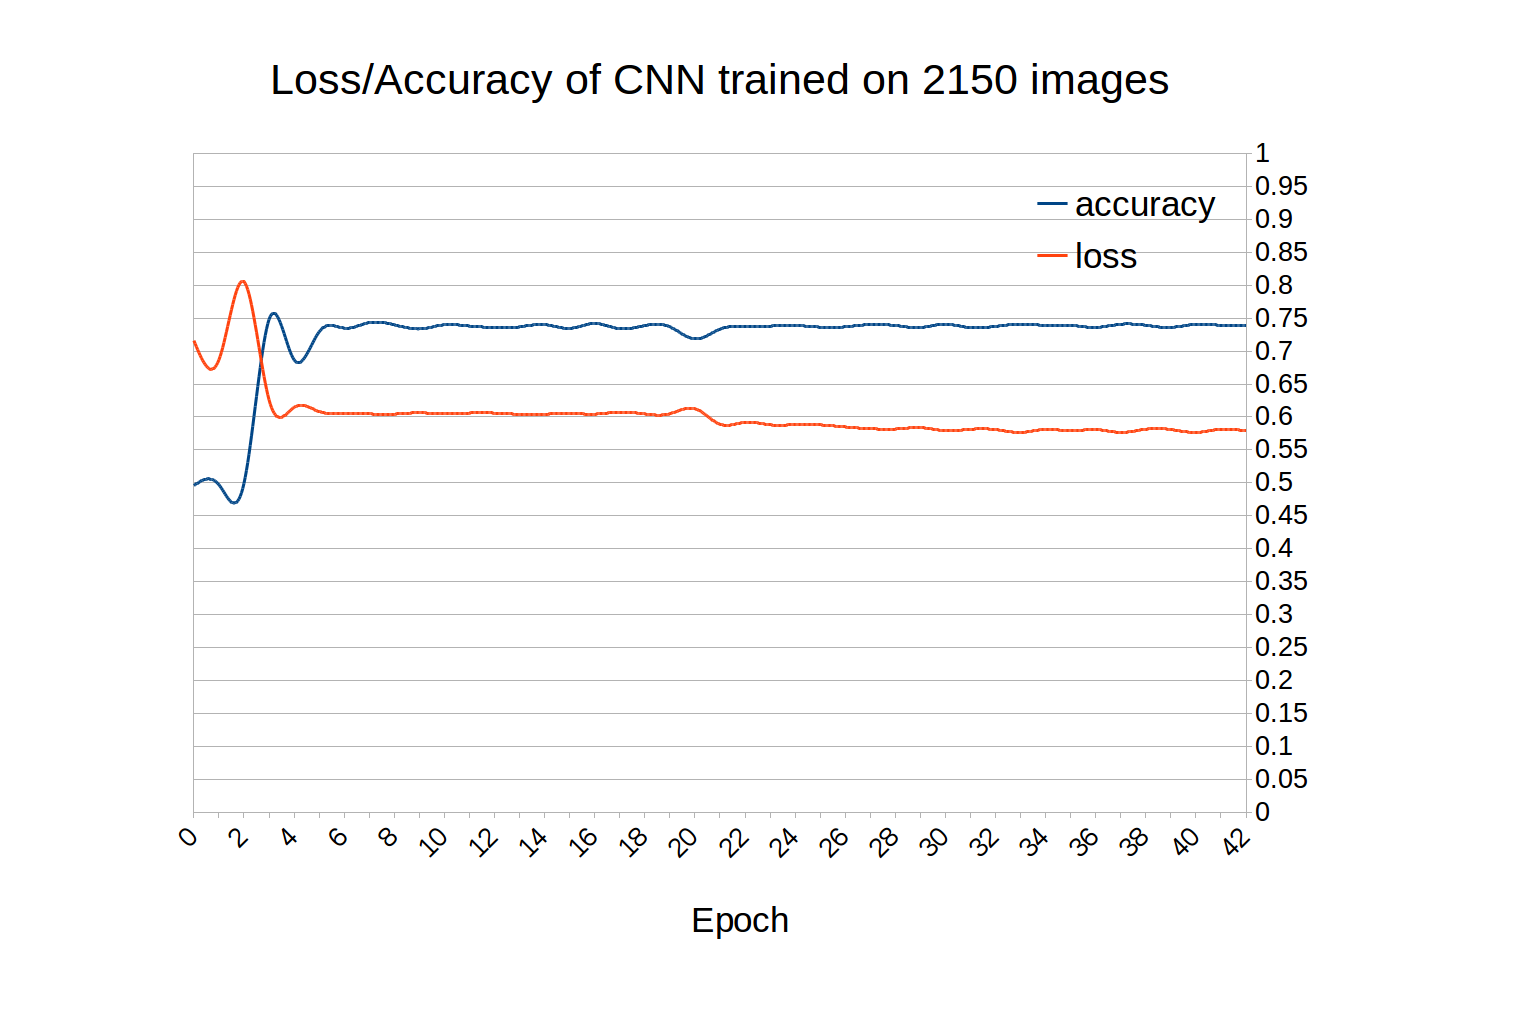
\includegraphics[width=\textwidth]{figs/acc_loss_CNN1075.png}
\caption{Accuracy vs. Loss of ImageNet 2-output $\mu/\pi$ sample consisting of 2,150 images each.} 
\label{fig:loss_accuracy_1075}
\end{figure}

The confusion matrices shown in figure \ref{fig:confusion1075} show the accuracy for both the training and testing datasets. The fact that these two have similar accuracies is important because if the training dataset had a much higher accuracy, that indicates an over-training of the training sample which means the neural network didn't learn features to separate muons from pions, it just memorized what was in the training dataset. Also note that the neural network does a better job of identifying muons than pions. This can be attributed to the more complex event scenes pions tend to leave in the detector due to pion interacting more in LAr than muons do. The CNN may do better at identifying pions with a larger training sample.

\begin{figure}[htp!]
\centering
	\begin{subfigure}[b]{.68\textwidth}
	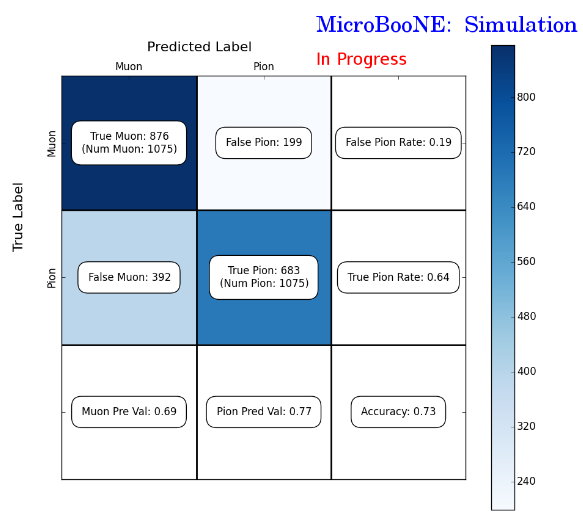
\includegraphics[width=\textwidth,height=3in]{figs/confusion1_train.png}
	\caption{Confusion Matrix showing Accuracy of CNN1075 using training MC data}
	\end{subfigure}
	\quad
	\begin{subfigure}[b]{.6\textwidth}
	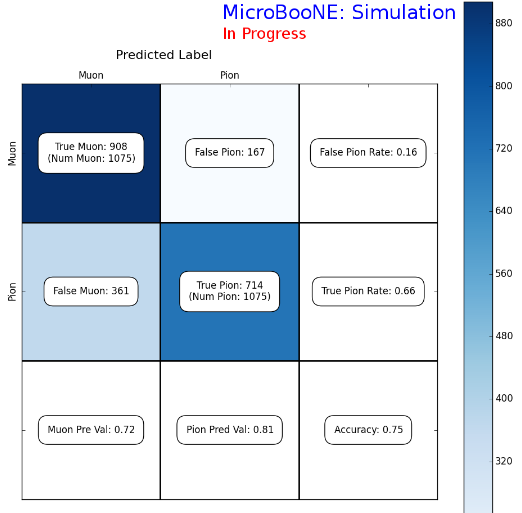
\includegraphics[width=\textwidth,height=3in]{figs/confusion1_test.png}
	\caption{Confusion Matrix showing Accuracy of CNN1075 using testing MC data}
	\end{subfigure}
	\quad
\caption{Description of confusion matrix varables: False pion rate = $false \pi/ total \pi$ True pion rate = $true \pi/total \pi$ Accuracy = $(true \pi rate + true \mu rate)/2$ Pion prediction value = $true \pi/(true \pi + false \pi)$ Muon prediction value = $true \mu/(true \mu + false \mu)$}
\label{fig:confusion1075}
\end{figure}

\subsection{Training CNN10000}
The hyperparameters used for CNN10000 are shown below. The batch size for the training and testing as well as the test{\_}iter were chosen to encompass the whole training/testing image set when doing accuracy/loss calculations. To do this, multiplying the test{\_}iter by the test batch size gives you the amount of images used when calculating accuracy/loss curves. 

\begin{multicols}{2}
\begin{itemize}
 \item \textit{train{\_}batch{\_}size: 100}
 \item \textit{test{\_}batch{\_}size: 100}
 \item \textit{test{\_}iter: 100}
 \item \textit{test{\_}interval: 100}
 \item \textit{base{\_}lr: 0.001}
 \item \textit{lr{\_}policy: "step"}
 \item \textit{gamma: 0.1}
 \item \textit{stepsize: 1000}
 \item \textit{display: 100}
 \item \textit{max{\_}iter: 10000}
 \item \textit{momentum: 0.99}
 \item \textit{weight{\_}decay: 0.0005}
 \item \textit{snapshot: 100}
\end{itemize}
\end{multicols}

The same architecure that was used to train CNN1075 was employed on CNN10000, AlexNet. Caffe \cite{caffe} was the software package used for both CNNs. The differences include batch size and test{\_}iter and momentum to account for the larger dataset. Figure \ref{fig:loss_accuracy} shows the loss and accuracy of CNN10000. There is around a 10\% increase in accuracy from CNN1075 to CNN10000, 85\%, and around a 20\% decrease in loss, 36\%.
\begin{figure}[htp!]
\centering
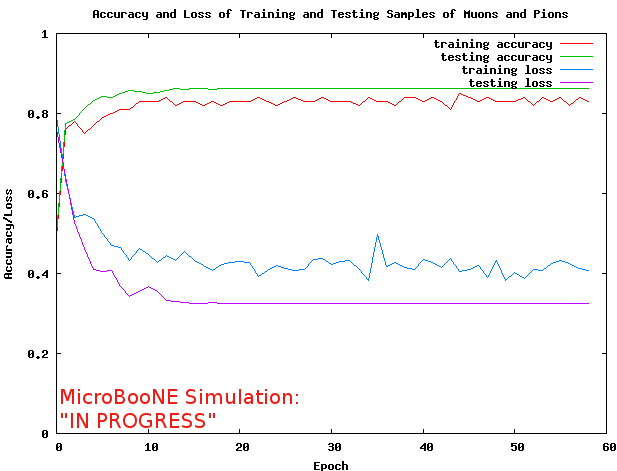
\includegraphics[width=\textwidth]{figs/acc_loss_10000_062117.png}
\caption{Accuracy vs. Loss of ImageNet 2-output $\mu/\pi$ sample consisting of 10,000 images each.} 
\label{fig:loss_accuracy}
\end{figure}

\begin{figure}[htp!]
\centering
	\begin{subfigure}[b]{.7\textwidth}
	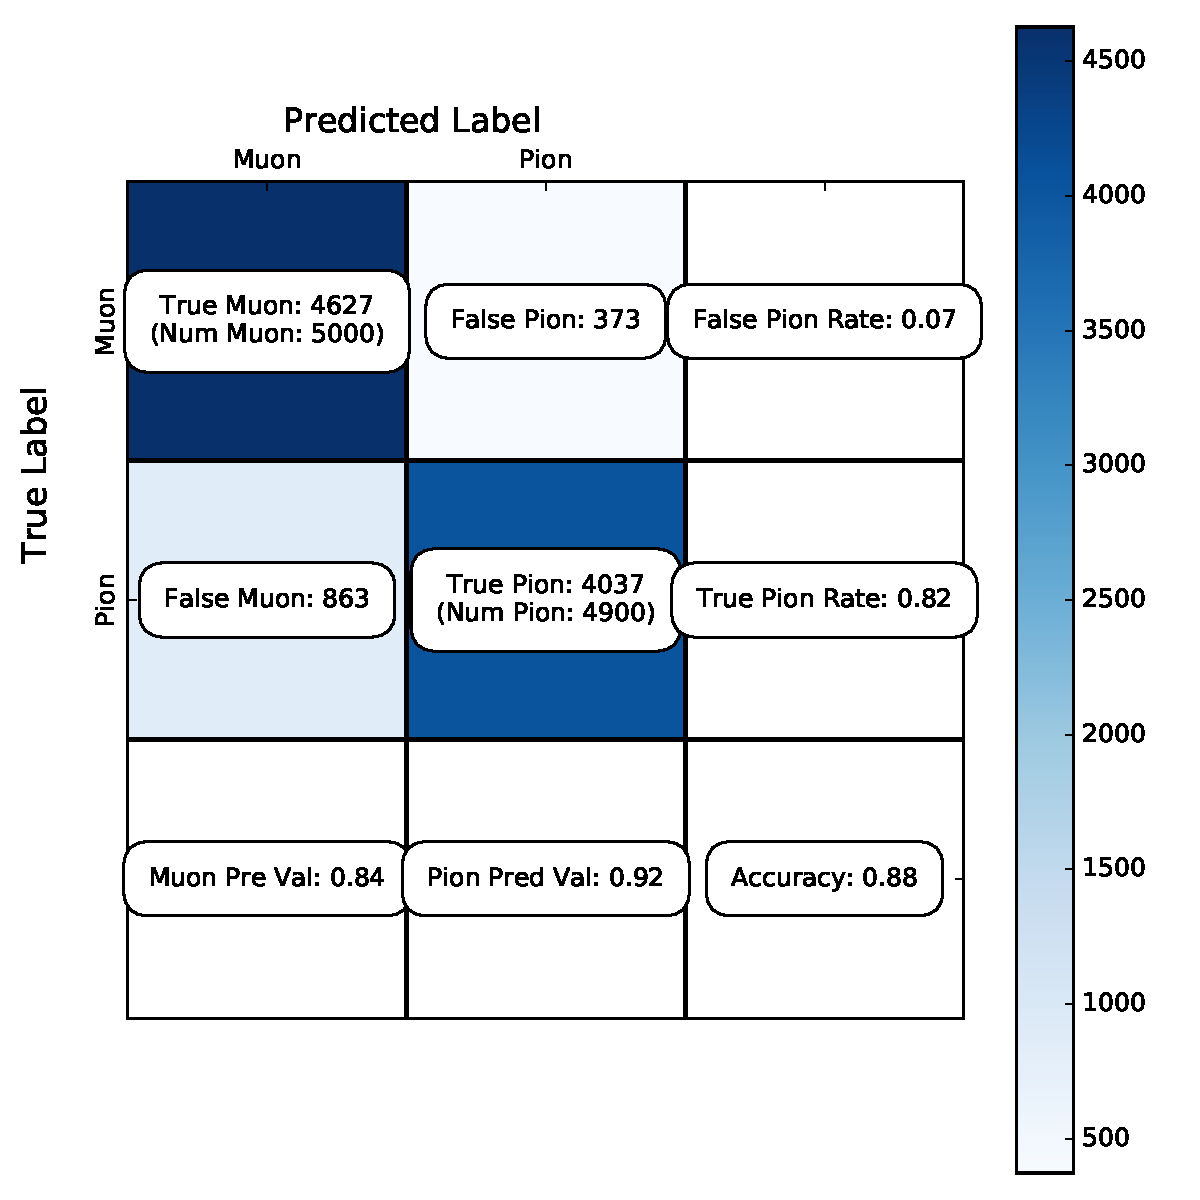
\includegraphics[width=\textwidth,height=3.5in]{figs/train_confusion.pdf}
	\caption{Confusion Matrix showing Accuracy of CNN10000 using training MC data}
	\label{fig:confusion}
	\end{subfigure}
	\quad
	\begin{subfigure}[b]{.7\textwidth}
	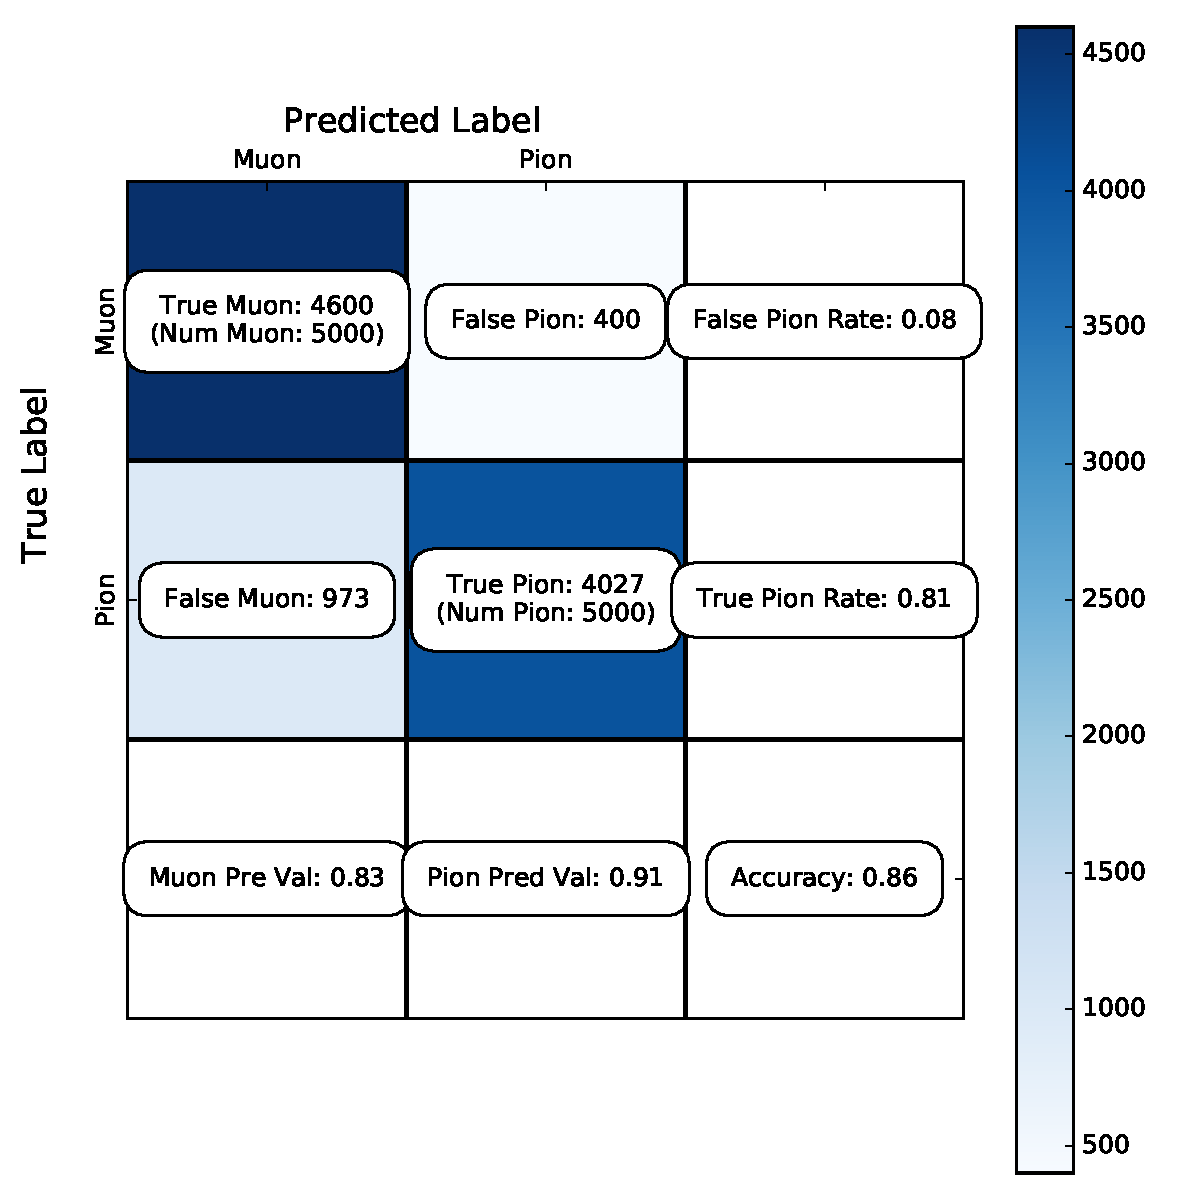
\includegraphics[width=\textwidth,height=3.5in]{figs/val_confusion.pdf}
	\caption{Confusion Matrix showing Accuracy of CNN10000 using testing MC data}
	\label{fig:confusion_test}
	\end{subfigure}
	\quad
\caption{Description of confusion matrix varables: False pion rate = $false \pi/ total \pi$ True pion rate = $true \pi/total \pi$ Accuracy = $(true \pi rate + true \mu rate)/2$ Pion prediction value = $true \pi/(true \pi + false \pi)$ Muon prediction value = $true \mu/(true \mu + false \mu)$}
\label{fig:CNN_train}
\end{figure}
\begin{figure}[htp!]
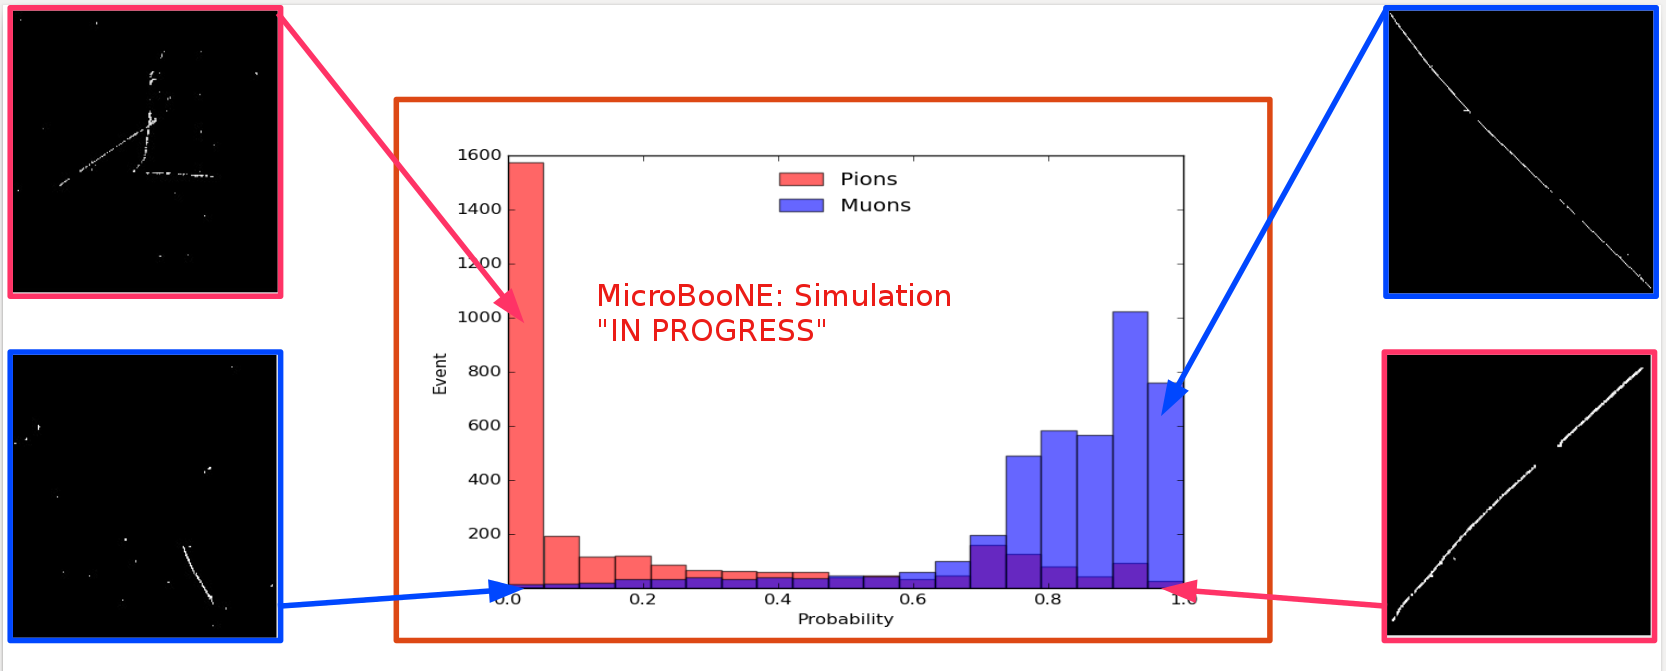
\includegraphics[width=\textwidth]{figs/mitch_hw.png}
\caption{Probability plot of muons and pions from testing set. Images surrounding histogram are a random event from lowest bin and highest bin for each particle.}
\label{fig:prob_plot}
\end{figure}

Figure \ref{fig:CNN_train} show a breakdown of $\mu/\pi$ separation for CNN10000. It also shows the network is not being overtrained due to the Accuracy of both the training and testing datasets being within .01\% of eachother. The CNN is doing a very good job of classifying true muons as muons, and our loss increase from CNN1075 is due to the increase in accurately classifing pions as pions. 



\subsection{Training CNN100000}
CNN100000 used the GoogleNet architecture rather than the AlexNet architecture used in the two previous trained CNNs. This is the first time the neural network was trained on a larger particle class, $\mu/\pi/p/\gamma/e$, and on higher resolution images. This CNN also employed GPUs during the training process. The hyperparameters are shown below:

\begin{multicols}{2}
\begin{itemize}
 \item \textit{train{\_}batch{\_}size: 18}
 \item \textit{test{\_}batch{\_}size: 2}
 \item \textit{test{\_}iter: 2000}
 \item \textit{test{\_}interval: 2000}
 \item \textit{base{\_}lr: 0.001}
 \item \textit{lr{\_}policy: "step"}
 \item \textit{gamma: 0.96}
 \item \textit{stepsize: 10000}
 \item \textit{average{\_}loss: 40}
 \item \textit{display: 40}
 \item \textit{max{\_}iter: 10000}
 \item \textit{momentum: 0.99}
 \item \textit{weight{\_}decay: 0.0002}
 \item \textit{snapshot: 50000}
\end{itemize}
\end{multicols}


\begin{figure}[htp]
\centering
\includegraphics[width=.8\linewidth=]{../images/GPU_9010split_hires_iterations_alldata_allparticle.png}
\caption{Training and testing accuracy of CNN trained on 100,000 images of \mu/\pi/p/\gamma/e with 20,000 images of each particle. Each image was a size of 576x576 and the images per particle were split 90\% use for training and 10\% used for testing the network}
\label{fig:gpuacc}
\end{figure}

\begin{figure}[htp]
\centering
\includegraphics[width=.8\linewidth=]{../images/GPU_9010split_hires_iterations_alldata_allparticle_loss.png}
\caption{Training and testing loss oc CNN trained on 100,000 images of \mu/\pi/p/\gamma/e}
\label{fig:gpuloss}
\end{figure}

\begin{figure}[htp]
\centering
\includegraphics[width=\linewidth=]{../images/confusion_allparticle_v3.pdf}
\caption{Confusion Matrix of all five particles }
\label{fig:confusion100000}
\end{figure}

\begin{figure}[htp]
\centering
\includegraphics[width=.8\linewidth=]{../csv_output/true_labels_1102.png}
\caption{t-SNE of CNN}
\label{fig:tsne}
\end{figure}

\begin{figure}[htp]
\centering
\includegraphics[width=.8\linewidth=]{../csv_output/muon_prob.png}
\caption{Muon Prob}
\label{fig:muonprob}
\end{figure}

\begin{figure}[htp]
\centering
\includegraphics[width=.8\linewidth=]{../csv_output/pi_prob.png}
\caption{Pion Prob}
\label{fig:piprob}
\end{figure}

\begin{figure}[htp]
\centering
\includegraphics[width=.8\linewidth=]{../csv_output/proton_prob.png}
\caption{Proton Prob}
\label{fig:protonprob}
\end{figure}

\begin{figure}[htp]
\centering
\includegraphics[width=.8\linewidth=]{../csv_output/eminus_prob.png}
\caption{Electron Prob}
\label{fig:eminusprob}
\end{figure}

\begin{figure}[htp]
\centering
\includegraphics[width=.8\linewidth=]{../csv_output/gamma_prob.png}
\caption{Gamma Prob}
\label{fig:gammaprob}
\end{figure}

\begin{figure}[htp]
\centering
\includegraphics[width=.8\linewidth=]{../csv_output/prob_allparticle_normalized.pdf}
\caption{Prob}
\label{fig:prob}
\end{figure}

\begin{figure}[htp]
\centering
\includegraphics[width=.8\linewidth=]{../csv_output/mu_pi_acc_tracklength_all.pdf}
\caption{mupi}
\label{fig:mu_pi}
\end{figure}

\begin{figure}[htp]
\centering
\includegraphics[width=.8\linewidth=]{../csv_output/mu_pi_acc_tracklength_75.pdf}
\caption{mupi}
\label{fig:mu_pi}
\end{figure}

\begin{figure}[htp]
\centering
\includegraphics[width=.8\linewidth=]{../csv_output/mu_pi_acc_momentum.pdf}
\caption{mupi}
\label{fig:mu_pi}
\end{figure}

\begin{figure}[htp]
\centering
\includegraphics[width=.8\linewidth=]{../csv_output/mu_p_acc_tracklength_all.pdf}
\caption{mup}
\label{fig:mu_p}
\end{figure}

\begin{figure}[htp]
\centering
\includegraphics[width=.8\linewidth=]{../csv_output/mu_p_acc_tracklength_75.pdf}
\caption{mup}
\label{fig:mu_p}
\end{figure}

\begin{figure}[htp]
\centering
\includegraphics[width=.8\linewidth=]{../csv_output/mu_p_acc_momentum.pdf}
\caption{mup}
\label{fig:mu_p}
\end{figure}

\begin{figure}[htp]
\centering
\includegraphics[width=.8\linewidth=]{../csv_output/mu_e_acc_tracklength_all.pdf}
\caption{mue}
\label{fig:mu_e}
\end{figure}

\begin{figure}[htp]
\centering
\includegraphics[width=.8\linewidth=]{../csv_output/mu_e_acc_tracklength_75.pdf}
\caption{mue}
\label{fig:mu_e}
\end{figure}

\begin{figure}[htp]
\centering
\includegraphics[width=.8\linewidth=]{../csv_output/mu_e_acc_momentum.pdf}
\caption{mue}
\label{fig:mu_e}
\end{figure}

\begin{figure}[htp]
\centering
\includegraphics[width=.8\linewidth=]{../csv_output/mu_g_acc_tracklength_all.pdf}
\caption{mug}
\label{fig:mu_g}
\end{figure}

\begin{figure}[htp]
\centering
\includegraphics[width=.8\linewidth=]{../csv_output/mu_g_acc_tracklength_75.pdf}
\caption{mug}
\label{fig:mu_g}
\end{figure}

\begin{figure}[htp]
\centering
\includegraphics[width=.8\linewidth=]{../csv_output/mu_g_acc_momentum.pdf}
\caption{mug}
\label{fig:mu_g}
\end{figure}

